\section{Introduction}\label{sec:intro}

\subsection{Motivation}
Suppose an analyst has a few hundred measurements and wants to know whether they come from one population or from a mixture of two. A histogram with two humps suggests two groups, but histograms show humps by chance, so the analyst wants a test. The usual choice is the dip test of Hartigan and Hartigan \cite{HH85}. It measures how far the empirical distribution function is from the nearest unimodal distribution function, and it rejects unimodality when that distance, the dip, is large. It needs no bandwidth and no parametric model, it is available in the R package \texttt{diptest} \cite{Maechler}, and clustering methods call it to decide whether a group should be split \cite{Maurus16,Bauer23}.

Whether the dip is ``large'' depends on what a unimodal law usually produces, and that depends on which unimodal law generated the data. Hartigan and Hartigan dealt with this by calibrating at one law. They took critical values from the uniform distribution and stated, in their abstract, that the uniform is asymptotically the least favourable unimodal distribution: among unimodal laws, it is supposed to produce the largest dips. If that holds, the uniform critical values are safe for every unimodal null, and conservative for most. Cheng and Hall \cite{CH98} later quantified the conservative side: for smooth laws with a well-defined peak, the rejection rate of the uniform-calibrated test tends to zero as the sample grows. Practitioners have reasonable grounds, then, to treat the uniform calibration as cautious.

\subsection{A unimodal law that the standard test rejects too often}
It is not cautious for every unimodal law. Consider the two-step density that spreads 90 percent of the mass evenly over $(0,0.995)$ and puts the remaining 10 percent on the narrow interval $(0.995,1)$. This law is unimodal: its density rises once, at $0.995$, and never falls back. \Cref{fig:fixedlaw} shows how often the standard 5 percent dip test rejects samples from it. At $n=200$ the rate is already 26 percent, and it stays near 25 percent up to $n=12{,}800$, the largest size we simulated. At the 1 percent level the rate settles near 10 percent. The same samples tested with the cutoff we propose are rejected at most about 3 percent of the time at the 5 percent level and 0.5 percent of the time at the 1 percent level.

\begin{figure}[t]
\centering
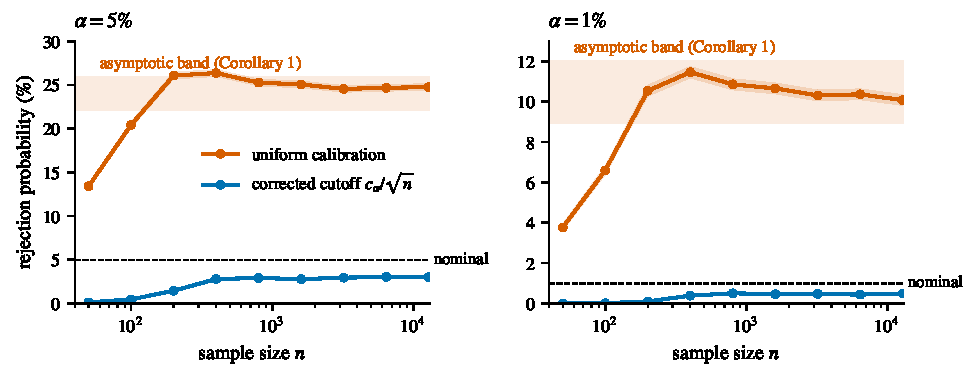
\includegraphics[width=\linewidth]{figs/fig3_fixed_law.pdf}
\caption{For this unimodal law the standard dip test rejects about a quarter of the samples at the nominal 5 percent level, and the excess does not shrink as $n$ grows. Rejection rates for the law with 90 percent of the mass spread evenly on $(0,0.995)$ and 10 percent on $(0.995,1)$, as the sample size grows. Orange: the standard dip test with uniform critical values. Blue: the constant cutoff $c_\alpha/\sqrt n$ proposed in \cref{sec:size}. Each point uses $50{,}000$ samples; the shaded strips around the lines are 95 percent intervals. The orange band is the asymptotic lower bound of \cref{cor:shoulder}, evaluated over the certified range of the limiting uniform critical value. The rejection rate of the standard test does not fall back towards the nominal level as $n$ grows.}
\label{fig:fixedlaw}
\end{figure}

Hartigan and Hartigan knew that the uniform is not least favourable at $n=4$; their paper gives a counterexample at that sample size \cite[p.~73]{HH85}. Müller \cite{Mueller92} suspected that certain bi-uniform laws are worse than the uniform, and Mächler's vignette for \texttt{diptest} calls the uniform ``not quite'' least favourable. None of these works shows a failure in large samples or measures how large it can be. \Cref{fig:fixedlaw} is a failure in large samples, and the rest of this paper explains it and gives a cutoff that removes it.

\subsection{The mechanism in brief}
It helps to keep two pictures side by side. A unimodal density rises to a peak and then falls. Its distribution function, which is what the dip test works with, therefore rises with increasing slope up to the peak, so it curves upward (is convex) there, and rises with decreasing slope after the peak, so it curves downward (is concave). We call the point where the curvature changes from upward to downward the \emph{turning point} of the distribution function; it sits at the mode of the density. To compute the dip, one looks for the unimodal distribution function closest to the empirical one, and that fit may put its turning point anywhere. Under the uniform law the fit uses this freedom: it bends wherever the random fluctuations of the sample make bending cheapest. The two-step law takes the freedom away. Its density jumps up at $0.995$, so the distribution function becomes much steeper there, and any fit that stays close to it must still be steepening at $0.995$. A unimodal fit stops steepening at its turning point, so the turning point of every close fit has to lie in the narrow top, and over the whole long flat part the fit has to curve upward. The random fluctuations of the empirical distribution function on that flat part look, at scale $n^{-1/2}$, like a Brownian bridge, and the best upward-curving (convex) fit to a Brownian bridge misses it by half the largest gap between the bridge and its greatest convex minorant. That half-gap is stochastically larger than the uniform limit of the dip, and this is why the test rejects too often. \Cref{sec:mechanism} turns this paragraph into a theorem.

\subsection{Contributions}
\begin{enumerate}[label=(\arabic*),leftmargin=*]
\item \emph{The failure.} For every level $\alpha\in(0,1)$ there is a fixed two-step unimodal law whose rejection probability under the uniform calibration stays above $\alpha$ by a fixed margin for all large $n$. The proof uses no numerical input (\cref{sec:mechanism}).
\item \emph{Its size.} Over atomless unimodal laws on a bounded interval with finite density at the mode, no law has a limiting rejection rate above $1-F_M(2\qbar_\alpha)$ under the standard test, and some laws come arbitrarily close to it. Here $F_M$ is the distribution function of the Balabdaoui--Pitman gap and $\qbar_\alpha$ is the limiting uniform critical value. Numerically this is 28.4 to 33.2 percent at the 5 percent level and 12.7 to 16.8 percent at 1 percent (\cref{sec:size}).
\item \emph{The correction.} The cutoff $c_\alpha/\sqrt n$, with $c_\alpha=\tfrac12F_M^{-1}(1-\alpha)$, keeps the limiting rejection rate at or below $\alpha$ for every law in that class, and no deterministic sequence of cutoffs with a smaller limit does (\cref{sec:size}).
\item \emph{The worst case at a given sample size.} We show that for every $n$, the rejection probability under any continuous unimodal law is at most that of a uniform sample whose fit is forced to turn at a fixed point. With this reduction and a computer-assisted argument we place the large-sample limit of the worst-case size in the same intervals as in (2) (\cref{sec:worst}).
\item \emph{Finite samples.} Certified cutoffs at $n=4$, at every $n$ from 8 to 49, and at six values of $n$ from 50 to 1600, together with enclosures of the size of the standard test at 21 sample sizes from 4 to 1000 (\cref{sec:finite}).
\item \emph{The cost.} The corrected test needs about twice the sample size of the uniform-calibrated test for the same power on symmetric normal mixtures, and in simulated clustering pipelines it removes most spurious splits of unimodal features that have flat parts (\cref{sec:practice}).
\end{enumerate}

\subsection{Scope and how the results were checked}
All results assume independent, identically distributed observations from a continuous distribution. Items (1) to (3) are theorems with written proofs. Item (4) combines proved reductions with a Monte Carlo certificate: a computation whose decision rule was fixed in advance and whose probability of certifying a false statement is bounded, by 0.01 or less in this paper. Items (2) to (4) also use the convergence of the scaled uniform critical values to $\qbar_\alpha$, which holds if the distribution function of the limiting uniform dip has neither a jump nor a flat stretch at $\qbar_\alpha$; we assume this, and simulation supports it (\cref{sec:setting}). The numerical constants are either enclosed rigorously by interval arithmetic or certified in the same Monte Carlo sense; \cref{sec:numbers} explains the difference. The deterministic steps of several arguments were also checked in the Lean proof assistant \cite{Lean4} with the Mathlib library \cite{Mathlib}. The code, the deposited outputs and the Lean files are in the repository named under the title.
